\section{Versuchsbeschreibung}

\subsection{Versuchsaufbau Normale Pendel}
\begin{figure}[H]
    \centering
    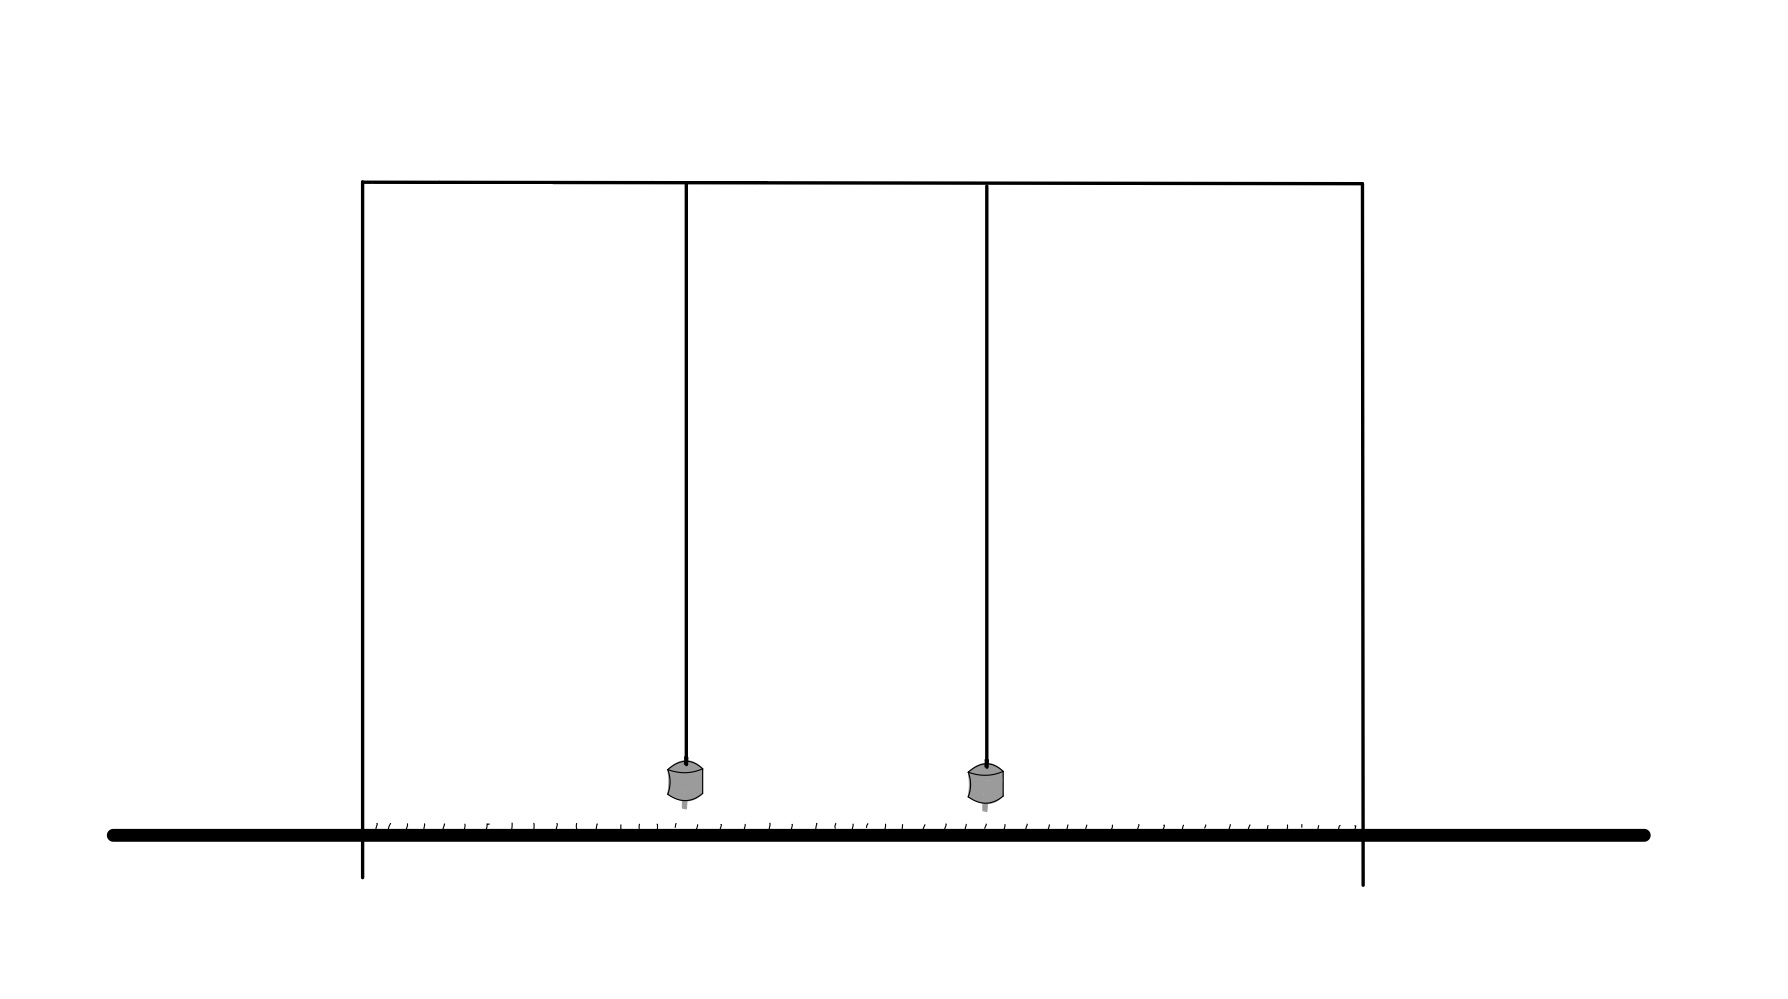
\includegraphics[width=\textwidth]{Bilder/Aufbau1.jpg}
    \caption{Eine selbst angefertigte Skizze des ersten Versuchsaufbau}
    \label{Aufbau1}
\end{figure}

Im ersten Teil des Versuches werden zwei Pendel benötigt die an einer Aufhängung schwingen können, zusätzlich wird ein Lineal benötigt mit welchem die Auslenkung der Pendel eingestellt werden kann als letztes wird eine Stoppuhr benötigt. Nun sollte der Aufbau ähnlich aussehen wie in Abbildung \ref{Aufbau1}.

\subsection{Versuchsaufbau Gekoppelte Pendel}

\begin{figure}[H]
    \centering
    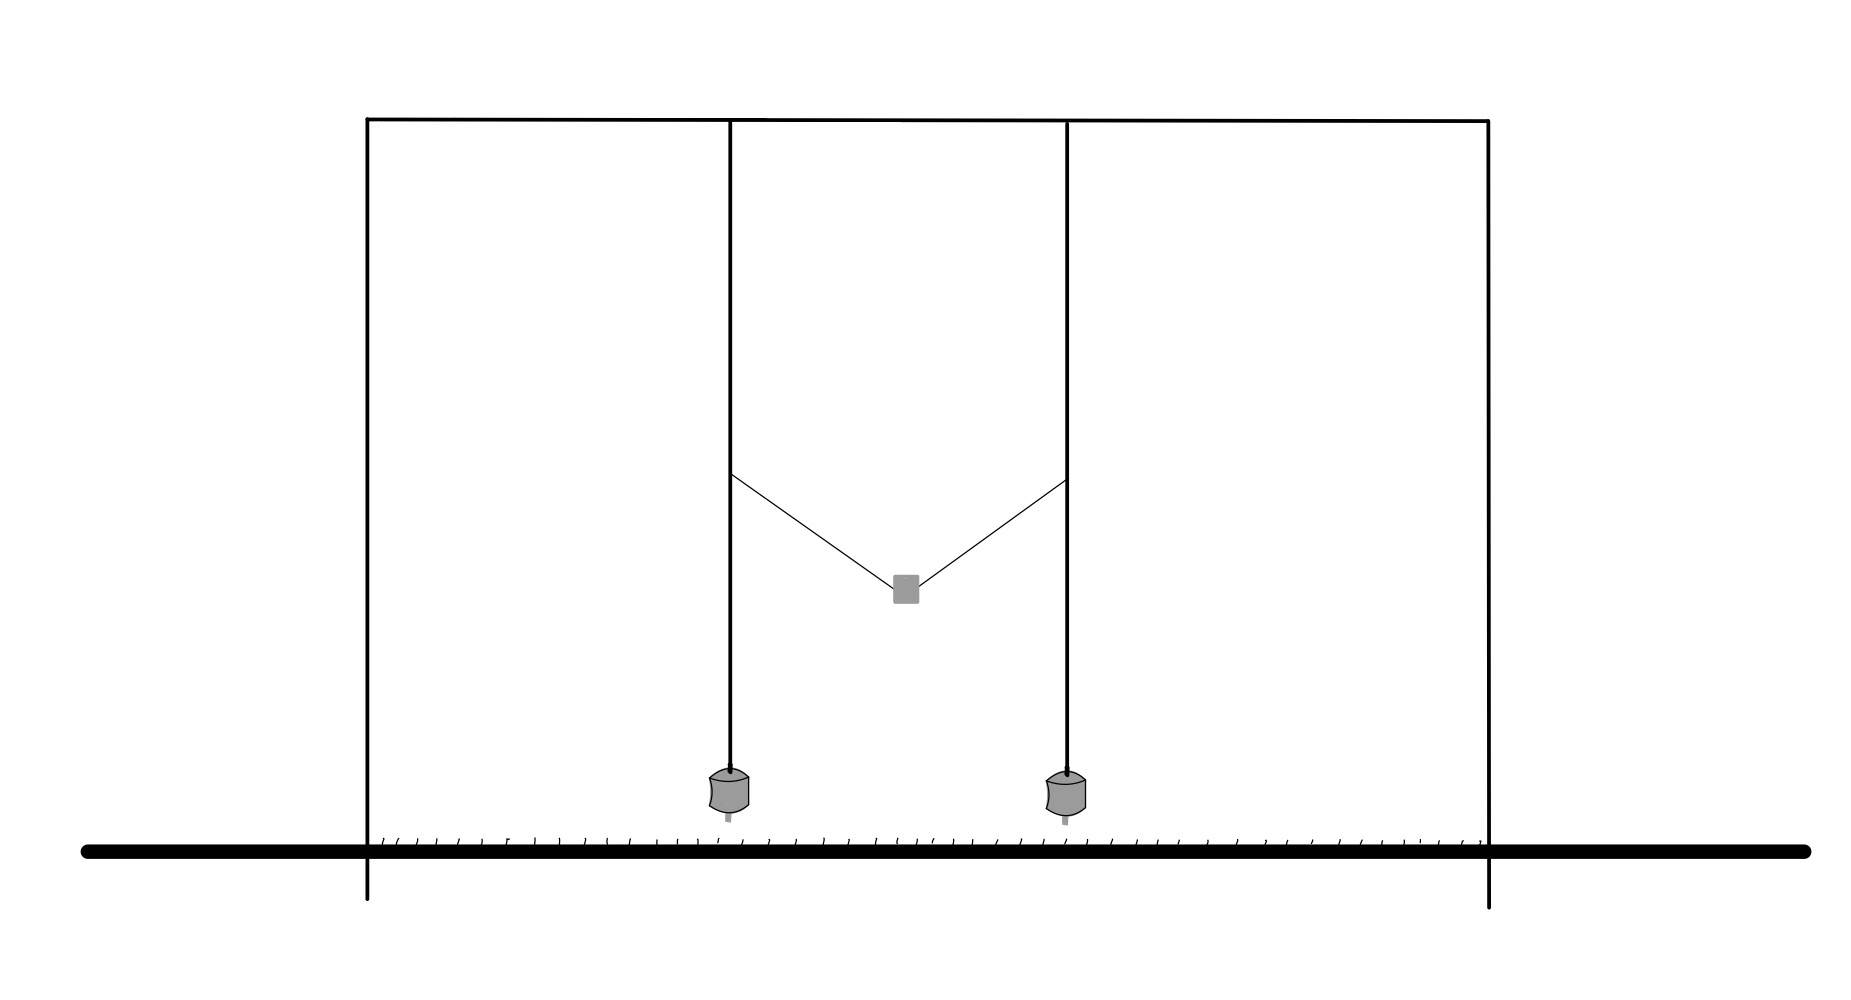
\includegraphics[width=\textwidth]{Bilder/Aufbau2.jpg}
    \caption{Eine selbst angefertigte Skizze des zweiten Versuchsaufbau}
    \label{Aufbau2}
\end{figure}
Für das gekoppelte Pendel wird nun ein Gewicht an Fäden benötigt womit dann die beiden Pendel so miteinander Verbunden werden dass das Gewicht genau in der Mitte der beiden Pendel hängt. Nun sollte der Aufbau wie in Abbildung \ref{Aufbau2} aussehen. 

\subsection{Versuchsdurchführung Teil 1}

\subsection{Versuchsdurchführung Teil 2}

\subsection{Versuchsdurchführung Teil 3}